\documentclass[10pt,draft]{article}

\usepackage{verbatim,multicol,color,amsmath,ifdraft, graphicx, wrapfig,setspace}

%\usepackage[latin1]{inputenc}
%\usepackage[T1]{fontenc}
%\usepackage[dvips]{graphicx}

\title{STAT 401A Mid-term Exam \\ Friday 19 October 8:00-8:50}
\author{Instructor: Jarad Niemi}
\date{}

\newenvironment{longitem}{
\begin{itemize}
  \setlength{\itemsep}{15pt}
  \setlength{\parskip}{20pt}
  \setlength{\parsep}{20pt}
}{\end{itemize}}

\setlength{\textheight}{9in}
\setlength{\textwidth}{6.5in}
\setlength{\topmargin}{-0.125in}
\setlength{\oddsidemargin}{-.2in}
\setlength{\evensidemargin}{-.2in}
\setlength{\headsep}{0in}

\newcommand{\bigbrk}{\vspace*{2in}}
\newcommand{\smallbrk}{\vspace*{.3in}}

\ifdraft{
  \newcommand{\correct}[1]{{\color{red} #1}}
  \newcommand{\shortcorrect}[1]{{\color{red} #1}}
  \newcommand{\longcorrect}[2][\bigbrk]{{\color{red} #2}}
}{
  \newcommand{\correct}[1]{}
  \newcommand{\shortcorrect}[1]{{\phantom{33.33}}}
  \newcommand{\longcorrect}[2][\bigbrk]{#1}
}

\newcommand{\iid}{\stackrel{iid}{\sim}}
\newcommand{\Yiid}{Y_1,\ldots,Y_n\stackrel{iid}{\sim}}

\begin{document}

\maketitle


\bigskip


\textbf{INSTRUCTIONS}

\bigskip

Please check to make sure you have 5 pages with writing on the front and back (some pages are marked `intentionally left blank'). Please remove the last page, i.e. the one with SAS code on front and back. When returned to you, the peer evaluation page will also be removed.

\bigskip

On the following pages you will find short answer questions related to the topics we covered in class for a total of 50 points. Please read the directions carefully.

\bigskip

You are allowed to use a calculator and one $8\frac{1}{2}\times 11$ sheet of paper with writing on both front and back. A non-exhaustive list of items you are not allowed to use are {\bf cell phones, laptops, PDAs, and textbooks}. Cheating will not be tolerated. Anyone caught cheating will receive an automatic F on the exam. In addition the incident will be reported, and dealt with according to University's Academic Dishonesty regulations. Please refrain from talking to your peers, exchanging papers, writing utensils or other objects, or walking around the room. All of these activities can be considered cheating. {\bf If you have any questions, please raise your hand.}

\bigskip

You will be given only the time allotted for the course; no extra time will be given.

\bigskip

Some notation that should be familiar:
\begin{center}
\begin{tabular}{ll}
%$Exp(\beta)$ &: exponential distribution with mean $\beta$ \\
%$Be(\alpha,\beta)$ &: beta distribution with parameters $\alpha$ and $\beta$ \\
%$Geo(p)$ &: Geometric distribution with probability of success $p$ \\
$t_v$ &: $t$-distribution with $v$ degrees of freedom \\
%$\chi^2_v$ &: $\chi^2$-distribution with $v$ degrees of freedom \\
$F_{u,v}$ &: $F$-distribution with $u$ numerator and $v$ denominator degrees of freedom \\
%$\chi^2_{v,\alpha}$ &: the value $c$ such that $P(X>c)=\alpha$ if $X\sim \chi^2_v$ \\
$t_{v}(a)$ &: the value $c$ such that $P(X<c)=a$ if $X\sim t_v$ \\
%$z_{\alpha}$ &: the value $c$ such that $P(X>c)=\alpha$ if $X\sim N(0,1)$ \\
$\overline{y}$ &= $\frac{1}{n} \sum_{i=1}^n y_i$ \\
$s_y^2$ &= $\frac{1}{n-1} \sum_{i=1}^n (y_i-\overline{y})^2$ \\
\end{tabular}
\end{center}

\smallbrk

Good Luck!

\smallbrk

Please print your name below:

\smallbrk


Student Name: \underline{\phantom{XXXXXXXXXXXXXXXXXXXXXXXXXXXXXXXXXXXXXXXXX}}  

\newpage

\noindent \begin{Large}Short answer (10 pts total) \end{Large}

\bigskip

One point will be awarded for a correct answer in each blank. 

\bigskip

\begin{enumerate}

\item If you are flipping a fair coin, what is the probability of observing the  sequence shown below? (1 pt)
\[ \mbox{T H T H T H T H H H} \]

\longcorrect[\vspace*{0.5in}]{$0.5^{10}\approx 0.001$}

\item If you are flipping a fair coin, what is the probability of observing the  sequence shown below? (1 pt)
\[ \mbox{H H H H H H H H H H} \]

\longcorrect[\vspace*{0.5in}]{$0.5^{10}\approx 0.001$}

\item Define pvalue. (2 pts)

\longcorrect[\vspace*{1in}]{The pvalue is the probability of observing a test statistic as or more extreme than that observed if the null hypothesis is true.}

\item What multiple comparison procedure can be used in any situation? (1 pt)

\longcorrect[\vspace*{0.5in}]{Bonferroni}

\item What one assumption does regression make in addition to the assumptions in ANOVA? (1 pt)

\longcorrect[\vspace*{0.5in}]{Linearity}

\item When is it appropriate to use the Wilcoxon rank-sum test? (2 pts)

\longcorrect[\vspace*{1.0in}]{When you have two unpaired samples with a similar distribution, but a normality assumption is unjustified.}

\item When is it appropriate to use Welch's t-test? (2 pts)

\longcorrect[\vspace*{0.8in}]{When you have two unpaired, normally-distributed samples with different variances.}

\end{enumerate}





\newpage
\noindent \begin{Large}Bird counts (10 pts total) \end{Large}

An experiment is conducted to determine the affect of logging practices on total bird counts. The total number of birds counted (sum) is recorded for four different logging treatments: dispersed (DT), large gap (LG), small gap (SG), and unharvested (zCL). 

Please answer the following questions {\bf based on the SAS code} titled ``Bird count''.

\begin{enumerate}
\item The ANOVA model is defined as 
\[ Y_{ij} \stackrel{ind}{\sim} N(\mu_i, \sigma^2), \quad i=1,\ldots,\mathrm{I} \]
where $Y_{ij}$ is the number of birds counted at location $j$ of treatment $i$. What is the value for $\mathrm{I}$ in this analysis? (1pt)

\longcorrect[\vspace*{0.5in}]{$\mathrm{I}=4$, there are 4 treatments}

\item What are the estimated values for each $\mu_i$ and for $\sigma^2$? (3 pts)

\longcorrect{$\mu_{DT} = 43.0, \mu_{LG}=40.6, \mu_{SG} = 38.3, \mu_{zCL}=25.8, \hat{\sigma}^2=239$ or $ \hat{\sigma}=15.4$ }

\item What is the interpretation for the pvalue in the ANOVA table, i.e. the one that corresponds to the F-statistic of 11.77? (2 pts)

\longcorrect[\vspace*{1in}]{This small pvalue means we reject the null hypothesis that all treatment means are the same.}

\item Conduct a hypothesis test to determine whether there is a difference between the dispersed treatment vs the large and small gap treatments combined. (2 pts)

\longcorrect[\vspace*{1.2in}]{We fail to reject the null hypothesis of no difference between dispersed vs large gap and small gap combined (p=0.2028). }


\item What is the interpretation of $R^2=0.158$? (2 pts)

\longcorrect[\vspace*{1in}]{15.8\% of the total variability is explained by allowing each treatment to have a different mean}


\end{enumerate}


\newpage
\noindent \begin{Large}Sea ice extent  (10 pts total) \end{Large}

\bigskip

One piece of evidence for global warming is decreased ice cover in the Arctic Ocean. Data were taken from Science magazine volume 337 page 1591 which plots the average August arctic sea ice extent, in million square kilometers, for the past 34 years. Running a regression of extent on year provides an estimate for when the Arctic Ocean will be \emph{ice-free}, defined to be less than 1 million square kilometers.

Please answer the following questions {\bf based on the SAS code} titled ``Sea ice extent''.

\begin{enumerate}
\item In statistical notation, write the model used in this analysis? (3 pts)\\
(Note: be sure to define any notation you introduce)

\longcorrect{\[Y_{i}\stackrel{ind}{\sim} N(\beta_0+\beta_1X_i,\sigma^2)\] where $Y_{i}$ represents the sea ice extent in millions of square kilometers and $X_i$ represents the year.} 

\item Provide an estimate for all parameters in the model above. (3 pts) \\

\longcorrect[\vspace*{.8in}]{$\hat{\beta}_0 = 159.9, \hat{\beta}_1 = -0.077, \hat{\sigma}^2 = 0.214$, or $\hat{\sigma} = 0.462$}

\item Provide a point estimate for when the Arctic Ocean will be ice-free, i.e. first hits 1 million square kilometers. (1 pt)

\shortcorrect{(1-159.9065)/(-0.07654) = 2076}\smallbrk

\item Provide a 95\% interval for when the Arctic Ocean will be ice-free. (3 pts)

\longcorrect{If $Y_0=1$ and from above $X_0=2076$, then we have 
\[ X_0 \pm t_{32}(1-\alpha/2) \frac{SE(Pred\{Y|X_0\})}{|\hat{\beta}_1|} \]
where 
\[ SE(Pred\{Y|X_0\}) = \hat{\sigma} \sqrt{1+\frac{1}{n}+\frac{(X_0-\overline{X})^2}{(n-1)s_X^2}} = 0.462 \sqrt{1+\frac{1}{34}+\frac{(2076-1995.5)^2}{(34-1)9.96^2}}=0.8013973\] 

Finally, using $t_{32}(1-\alpha/2)\approx 2$, we have
\[ 2076 \pm 2 \frac{0.801}{.077} = (2055,2097) \]
}

\end{enumerate}

\newpage
\noindent \begin{Large}Residual diagnostics  (10 pts total) \end{Large}

\bigskip 

\noindent The plots below are possible residual (y-axis) vs year (x-axis) plots for the Sea Ice Extent problem in the previous example. For each plot determine the type of violation, if there is one, indicated by the plot. Each of these possibilities are used exactly once: {\bf constant variance}, {\bf linearity}, {\bf independence}, {\bf heavy-tails}, and {\bf no violation}. (2 pts each)

\vspace{0.2in}

\begin{minipage}{0.6\linewidth}
    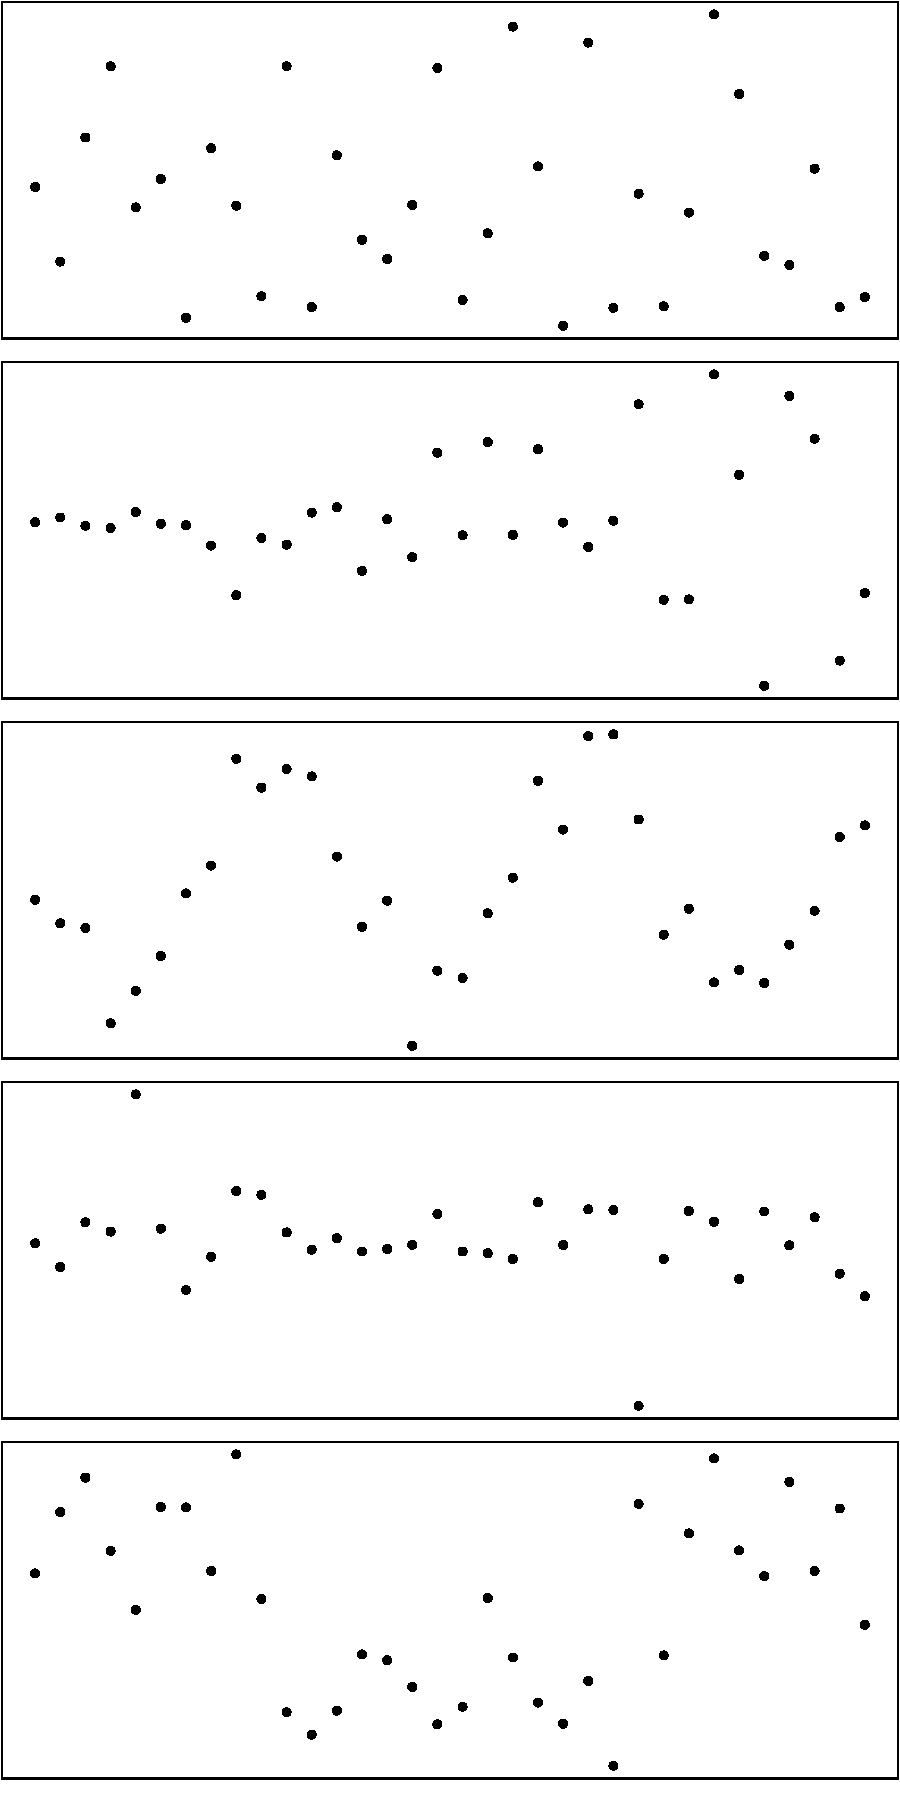
\includegraphics[width=\textwidth]{plots}
\end{minipage}
\begin{minipage}{0.4\linewidth}
{\Huge

\vspace{-0.2in}

A.\correct{No violation}

\vspace{1.2in}

B.\correct{Constant variance}

\vspace{1.2in}

C.\correct{Linearity/Independence}

\vspace{1.2in}

D.\correct{Heavy-tailed}

\vspace{1.2in}

E.\correct{Linearity/Independence}
}
\end{minipage}

\begin{comment}
\newpage
(intentionally left blank)

\newpage

\noindent \begin{Large}Mid-term peer evaluation  (10 pts total) 
\end{Large}

\bigskip

Please assign scores (higher is better) that reflect how you really feel about the extent to which the other members of your team contributed to your learning and/or your team's performance. This will be your only opportunity to reward the members of your team who worked hard on your behalf. (Note: If you give everyone pretty much the same score you will be hurting those who did the most and helping those who did the least.)

{\bf Instructions:} In the space below please rate each of the {\bf other} members of your team. Each member's peer evaluation score will be the average of the points they receive from the other members of the team. To complete the evaluation you should: 1) List the {\bf last name} of each member of your team in the alphabetical order of their last names and, 2) assign an average of ten points to the {\bf other} members of your team (Thus, for example, you should assign a total of 50 points in a six-member team; 60 points in a seven-member team; etc.) and, 3) differentiate some in your ratings; for example, you must give at least one score of 11 or higher (maximum=15) and one score of 9 or lower.

\vspace{0.2in}

{\Large
\begin{tabular}{l@{\qquad}c@{\qquad}c@{\qquad}l@{\qquad}c@{\qquad}c@{\qquad}}
& Team Members & Score & & Team Members & Score \\
\hline
1) & & & 5) & & \\
\hline
2) & & & 6) & & \\
\hline
3) & & & 7) & & \\
\hline
4) & & & 8) & & \\
\hline
\end{tabular}
}

\vspace{0.3in}

{\bf Additional Feedback:} In the space below would you also briefly describe your reasons for your highest and lowest ratings. These comments -- but not information about who provided them -- will be used to provide feedback to students who would like to receive it.

Provide at least {\bf one positive critique} and {\bf one area for improvement}.

\vspace{0.2in}

{\bf Positive critique:}

\vspace{2in}

{\bf Area of improvement:} 


\newpage
(intentionally left blank)
\end{comment}

\newpage
SAS Code - Bird count
\begin{verbatim}
PROC GLM DATA=birdcounts;
  CLASS overt;
  MODEL sum = overt;
  LSMEANS overt / ADJUST=TUKEY;
  ESTIMATE '1' overt 1  1  1 -3 / DIVISOR=3; 
  ESTIMATE '2' overt 2 -1 -1  0 / DIVISOR=2; 
  ESTIMATE '3' overt 0  1 -1  0;
  RUN;

                                        The GLM Procedure

Dependent Variable: sum

                                               Sum of
       Source                      DF         Squares     Mean Square    F Value    Pr > F
       Model                        3      8419.60417      2806.53472      11.77    <.0001
       Error                      188     44843.37500       238.52859
       Corrected Total            191     53262.97917

                       R-Square     Coeff Var      Root MSE      sum Mean
                       0.158076      41.82397      15.44437      36.92708
                                        
                                       Least Squares Means
                                      overt      sum LSMEAN

                                      DT         42.9583333
                                      LG         40.6041667
                                      SG         38.3333333
                                      zCL        25.8125000
                                                                     
                              Least Squares Means for effect overt
                              Pr > |t| for H0: LSMean(i)=LSMean(j)

                                    Dependent Variable: sum

                  i/j              1             2             3             4

                     1                      0.8780        0.4595        <.0001
                     2        0.8780                      0.8889        <.0001
                     3        0.4595        0.8889                      0.0006
                     4        <.0001        <.0001        0.0006


                                                       Standard
           Parameter                   Estimate           Error    t Value    Pr > |t|

           1                         14.8194444      2.57406181       5.76      <.0001
           2                          3.4895833      2.73020484       1.28      0.2028
           3                          2.2708333      3.15256899       0.72      0.4722
\end{verbatim}

\newpage
SAS Code - Sea ice extent
\begin{verbatim}
DATA arctic;
  INFILE 'arctic.csv' DSD FIRSTOBS=2;
  INPUT year extent;

PROC MEANS DATA=arctic;
  VAR extent year;

PROC REG DATA=arctic;
  MODEL extent = year;
  RUN;

                                       The MEANS Procedure

         Variable     N            Mean         Std Dev         Minimum         Maximum
         ------------------------------------------------------------------------------
         extent      34       7.1752941       0.8876808       4.8000000       8.4000000
         year        34         1995.50       9.9582462         1979.00         2012.00
         ------------------------------------------------------------------------------
                                      Analysis of Variance

                                             Sum of           Mean
         Source                   DF        Squares         Square    F Value    Pr > F

         Model                     1       19.17043       19.17043      89.78    <.0001
         Error                    32        6.83282        0.21353
         Corrected Total          33       26.00325


                      Root MSE              0.46209    R-Square     0.7372
                      Dependent Mean        7.17529    Adj R-Sq     0.7290
                      Coeff Var             6.43999


                                      Parameter Estimates

                                   Parameter       Standard
              Variable     DF       Estimate          Error    t Value    Pr > |t|

              Intercept     1      159.90650       16.11915       9.92      <.0001
              year          1       -0.07654        0.00808      -9.48      <.0001
\end{verbatim}


\end{document}

